\documentclass[border=10pt]{standalone}
\usepackage{tikz}
\usepackage{fontspec}
\usepackage{xcolor}

% Use TeX Gyre Termes (Times clone) which is available in all TeX distributions
\setmainfont{TeX Gyre Termes}
\setsansfont{TeX Gyre Heros}
\setmonofont{TeX Gyre Cursor}

% TikZ libraries
\usetikzlibrary{shapes,arrows,positioning,calc,patterns,decorations.pathreplacing,chains,shadows}
\usetikzlibrary{shapes.geometric,shapes.symbols,shapes.misc}
\usetikzlibrary{matrix,fit,backgrounds}
\usetikzlibrary{arrows.meta}

% Custom colors
\definecolor{bertblue}{RGB}{66,133,244}
\definecolor{gptgreen}{RGB}{52,168,83}
\definecolor{vitpurple}{RGB}{142,36,245}
\definecolor{maskred}{RGB}{234,67,53}
\definecolor{clsorange}{RGB}{251,188,5}
\definecolor{darkgray}{RGB}{50,50,50}
\definecolor{unkred}{RGB}{234,67,53}
\definecolor{subwordpurple}{RGB}{142,36,245}
\definecolor{sepviolet}{RGB}{142,36,245}

% Custom commands for special tokens
\newcommand{\specialtoken}[1]{\texttt{[#1]}}
\newcommand{\cls}{\specialtoken{CLS}}
\newcommand{\sep}{\specialtoken{SEP}}
\newcommand{\mask}{\specialtoken{MASK}}
\newcommand{\pad}{\specialtoken{PAD}}
\newcommand{\unk}{\specialtoken{UNK}}
\newcommand{\sos}{\specialtoken{SOS}}
\newcommand{\eos}{\specialtoken{EOS}}

\begin{document}
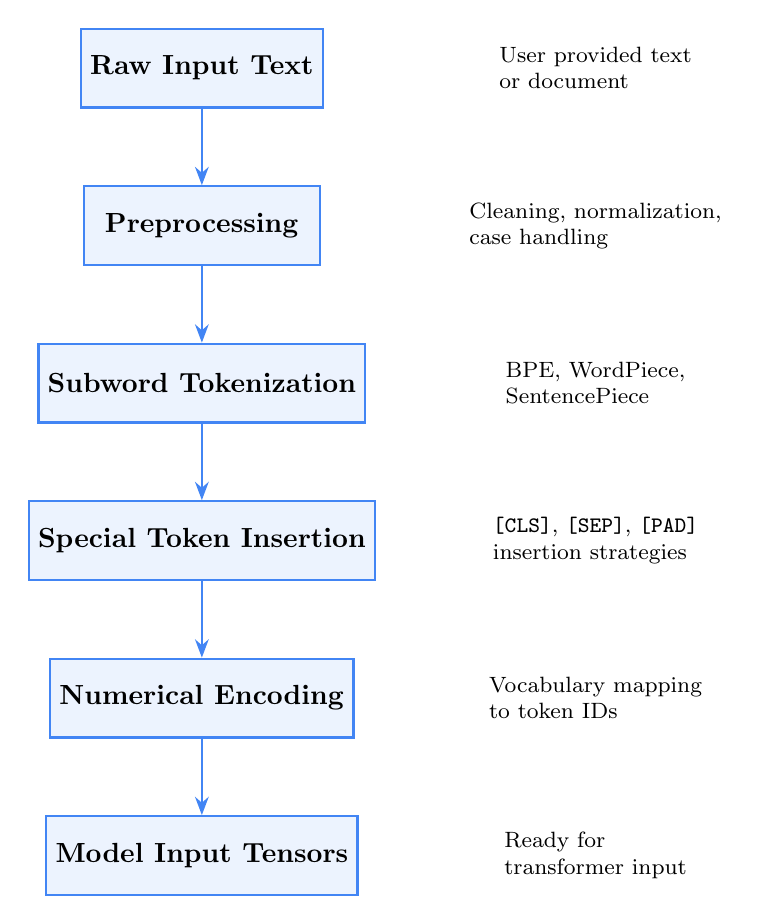
\begin{tikzpicture}[
    box/.style={rectangle, minimum width=3cm, minimum height=1cm, draw=bertblue, fill=bertblue!10, thick},
    arrow/.style={-{Stealth}, thick, bertblue},
    textnode/.style={font=\footnotesize}
]

% Pipeline stages
\node[box] (input) at (0, 0) {\textbf{Raw Input Text}};
\node[box] (preproc) at (0, -2) {\textbf{Preprocessing}};
\node[box] (tokenize) at (0, -4) {\textbf{Subword Tokenization}};
\node[box] (special) at (0, -6) {\textbf{Special Token Insertion}};
\node[box] (encode) at (0, -8) {\textbf{Numerical Encoding}};
\node[box] (output) at (0, -10) {\textbf{Model Input Tensors}};

% Arrows
\draw[arrow] (input) -- (preproc);
\draw[arrow] (preproc) -- (tokenize);
\draw[arrow] (tokenize) -- (special);
\draw[arrow] (special) -- (encode);
\draw[arrow] (encode) -- (output);

% Side annotations
\node[textnode, align=left] at (5, 0) {User provided text\\or document};
\node[textnode, align=left] at (5, -2) {Cleaning, normalization,\\case handling};
\node[textnode, align=left] at (5, -4) {BPE, WordPiece,\\SentencePiece};
\node[textnode, align=left] at (5, -6) {\cls{}, \sep{}, \pad{}\\insertion strategies};
\node[textnode, align=left] at (5, -8) {Vocabulary mapping\\to token IDs};
\node[textnode, align=left] at (5, -10) {Ready for\\transformer input};

\end{tikzpicture}
\end{document}